\documentclass[12pt,a4paper,twocolumn]{report}
\usepackage[utf8]{inputenc}
\usepackage{amsmath}
\usepackage{amsfonts}
\usepackage{amssymb}
\usepackage{graphicx}
\usepackage{float}
\begin{document}
\section*{Result}
Task started: \hfill 15:52 06-06-2017
\\
Task ended: \hfill 16:18 06-06-2017
\\
Total time consumed: 26 min on 1 tasks\\
\section*{Control}
XC  \hfill \textbf{pbe}\\
Relativistic  \hfill \textbf{atomic\textunderscore zora}\\
Charge  \hfill \textbf{1}\\
Max. number of iterations is \hfill \textbf{10000}\\
\textbf{Relaxation was performed\\}
\\
Other settings:\\
\\
vdw\textunderscore correction\textunderscore hirshfeld\\
sc\textunderscore accuracy\textunderscore rho    1E-4\\
sc\textunderscore accuracy\textunderscore eev    1E-3\\
sc\textunderscore accuracy\textunderscore etot   1E-6\\
sc\textunderscore accuracy\textunderscore forces 5E-4\\
\\
\newpage
\begin{figure}[h!]
\caption{Atoms: H, O, C, N, Na } 
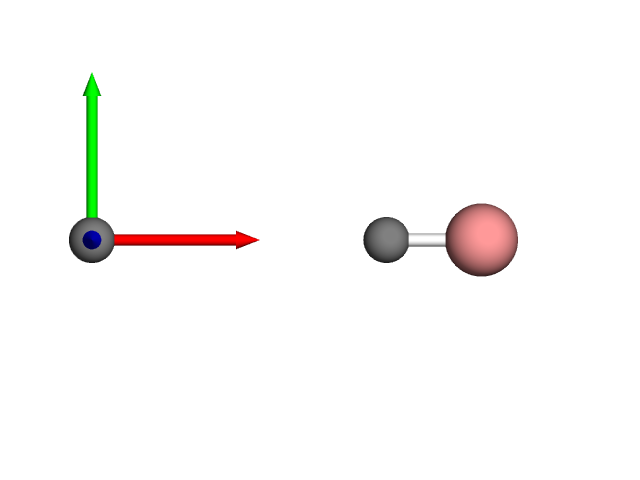
\includegraphics[width=0.6\textwidth]{geometry.png}
\end{figure}
\begin{figure}[H]
\caption{Energy convergence during geometry relaxation process.} 
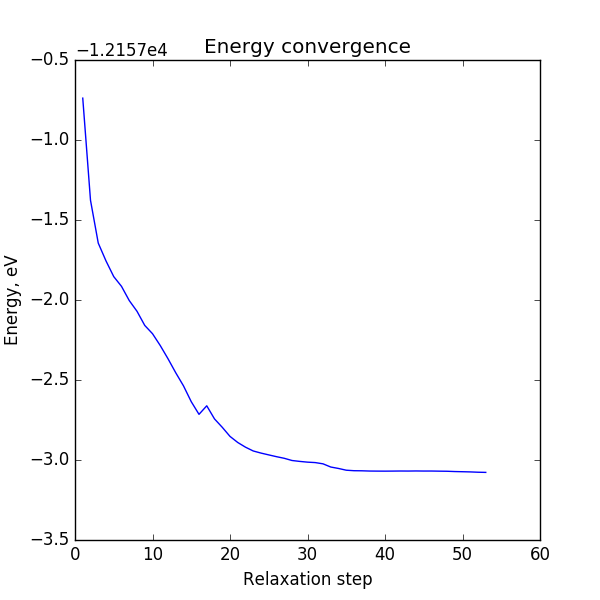
\includegraphics[width=0.5\textwidth]{energy_convergence.png}
\end{figure}
\end{document}